\section{Wind turbine models}
The two-bladed rotating \gls{WGTM}s are made at KTH Royal Institute of Technology in Stockholm, and can be seen in figure \ref{fig:rwtm}. They have a diameter of 45 \si{\mm}, and a hub height of approximately 65 \si{\mm}. Magnets are incorporated into the bottom of the models. 
%ADD PICTURE 


\begin{figure} 
    \centering
    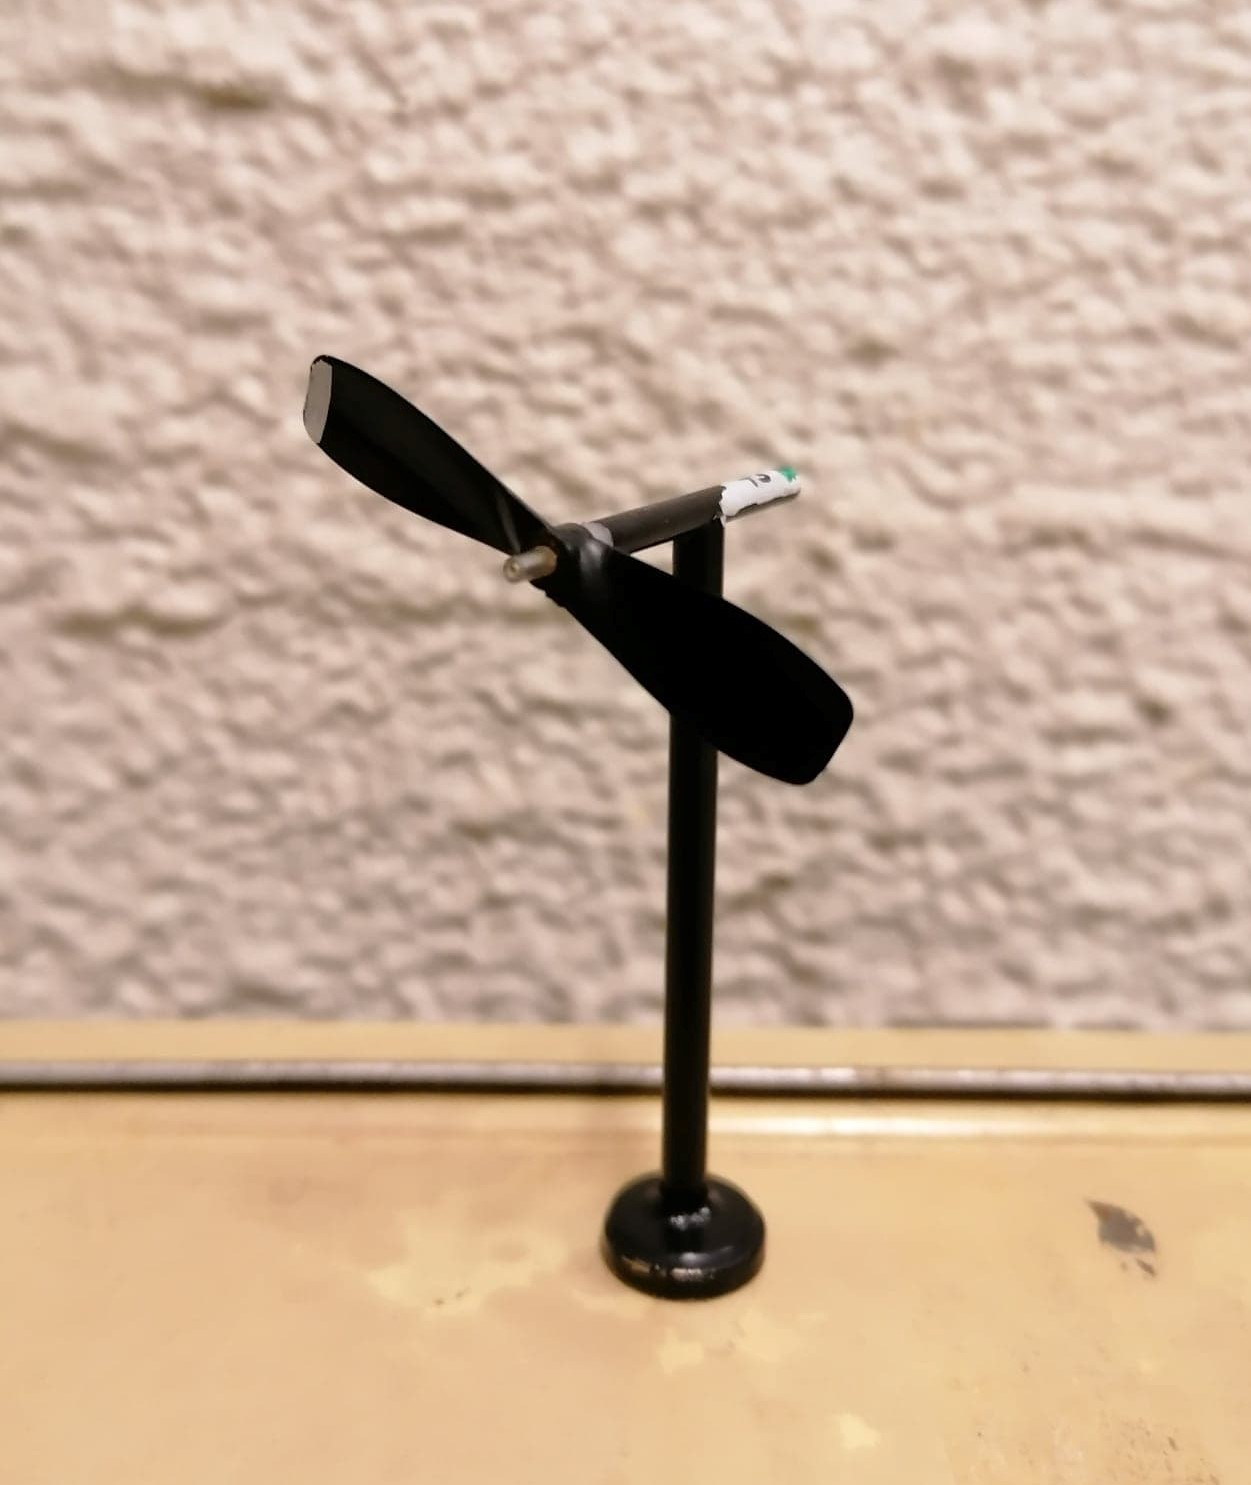
\includegraphics[width=0.5\textwidth]{0_Images/RWTM.jpg}    
    \caption{One of the rotating models.}
    \label{fig:rwtm}
\end{figure}

\FloatBarrier